\section{Motivating Example}
\label{sec:motivating-example}

In this section, we illustrate how our \textsc{MockDetector} tool finds a mock object created within a unit test case. Our tool identifies variables which have been assigned an object flowing from a mock creation site either through a forward flow may analysis (Soot-based analysis) or through specified declarative constraints (Doop-based analysis).

% explain focal methods first.

To motivate our work, consider Listing~\ref{lis:mockCall}, which presents a unit test case from the Maven project. Line 8 calls \textit{getRequest()}, invoking it on the mock object \texttt{session}. Line 12 then calls \textit{getToolchainsForType()}---this is the actual focal method whose behaviour is being tested. At the bytecode level, the two method invocations are indistinguishable with respect to mockness; to our knowledge, current static analysis tools cannot easily tell the difference between the method invocation on a mock object on line 8 and the method invocation on a real object on line 12. This uncertainty would confound, for instance, a naive static analysis that attempts to identify focal methods. Figure~\ref{fig:focalMethodIllustration} highlights our analysis tool's process in removing non focal method calls on mock objects.

While we were designing \textsc{MockDetector}, we observed several cases where mock objects are stored in arrays and collections. Listing~\ref{lis:container} presents method \textit{setUp()} in class \texttt{NodeListIteratorTest.java} from commons-collections-4.4, where line 9 puts the mock \textsc{Node} objects in the array-typed field \texttt{nodes}, which is later used in test cases. To find arrays containing mock objects, our analysis would first locate assignment statements containing array references, and would gather all the local variables or field references in these statements. It then checks whether any of these local variables or field references have already been marked as mock objects in the analysis. If so, then the tool would mark the local variable or field reference representing the array as an arrayMock, meaning that the mockness has propagated to this array container. Figure~\ref{fig:arrayMockIllustration} illustrates the process in finding mock-containing containers.

\lstset{language=java,
	keywordstyle=\color{blue}\bfseries,
	commentstyle=\color{green},
	stringstyle=\ttfamily\color{red!50!brown},
        showstringspaces=false}
\lstset{literate=%
	*{0}{{{\color{red!20!violet}0}}}1
	{1}{{{\color{red!20!violet}1}}}1
	{2}{{{\color{red!20!violet}2}}}1
	{3}{{{\color{red!20!violet}3}}}1
	{4}{{{\color{red!20!violet}4}}}1
	{5}{{{\color{red!20!violet}5}}}1
	{6}{{{\color{red!20!violet}6}}}1
	{7}{{{\color{red!20!violet}7}}}1
	{8}{{{\color{red!20!violet}8}}}1
	{9}{{{\color{red!20!violet}9}}}1
}

\begin{lstlisting}[basicstyle=\ttfamily, caption={This code snippet illustrates an example from maven-core, where both the focal method and a method invocation on a mock object occur in test \textit{testMisconfiguredToolchain()}},
basicstyle=\scriptsize\ttfamily,language = Java, framesep=4.5mm,
framexleftmargin=1.0mm, captionpos=b, xleftmargin=3.5ex, label=lis:mockCall]

@Test
public void testMisconfiguredToolchain() throws Exception {
	MavenSession session = mock( MavenSession.class );
	MavenExecutionRequest req = 
		new DefaultMavenExecutionRequest();
	when( session.getRequest() ).thenReturn( req );
	
	ToolchainPrivate[] basics =
	 	toolchainManager.getToolchainsForType("basic", session);
	
	assertEquals( 0, basics.length );
}

\end{lstlisting}

\begin{lstlisting}[basicstyle=\ttfamily, caption={This example illustrates a field array container holding mock objects from \textit{setup()} in \texttt{NodeListIteratorTest.java}.},
basicstyle=\scriptsize\ttfamily,language = Java, framesep=4.5mm, framexleftmargin=1.0mm, captionpos=b, xleftmargin=3.5ex, label=lis:container]

// Node array to be filled with mocked Node instances
private Node[] nodes;

@Test
protected void setUp() throws Exception {
	...
	
	// create mocked Node Instances and 
	// fill Node[] to be used by test cases
	final Node node1 = createMock(Element.class);
	final Node node2 = createMock(Element.class);
	final Node node3 = createMock(Text.class);
	final Node node4 = createMock(Element.class);
	nodes = new Node[] {node1, node2, node3, node4};
	...
}

\end{lstlisting}


\begin{figure}
	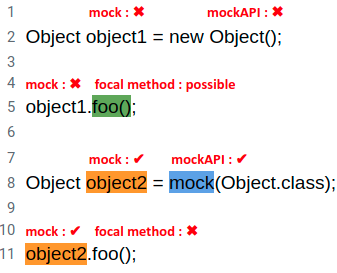
\includegraphics[width=.25\textwidth]{Images/mockFocalMethodIllustration.png}
	
	\caption{Illustration of the process locating mock object and determining non focal method.}
	\label{fig:focalMethodIllustration}
	
\end{figure}

\begin{figure}
	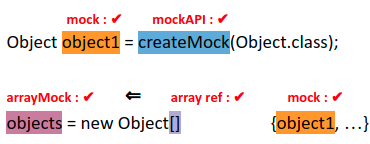
\includegraphics[width=.25\textwidth]{Images/arrayMockIllustration.png}
	
	\caption{Illustration of the process determining array that is an arrayMock.}
	\label{fig:arrayMockIllustration}
	
\end{figure}